%%% Uncomment the following for normal slide show
%
%\documentclass{beamer}

%%% or uncomment this for handouts
%\documentclass[handout,ignorenonframetext]{beamer}

%%% or uncomment this for the article version
\documentclass[11pt]{article}


\usepackage{beamerarticle}

%\usepackage{ru, url}

\usepackage[british]{babel}
\usepackage{listings, color, float, graphicx}
\definecolor{dkgreen}{rgb}{0,0.6,0}
\definecolor{gray}{rgb}{0.5,0.5,0.5}
\definecolor{mauve}{rgb}{0.58,0,0.82}
 

\lstset{frame=tb,
  language=Haskell,
  aboveskip=3mm,
  belowskip=3mm,
  showstringspaces=false,
  columns=flexible,
  basicstyle={\small\ttfamily},
  numbers=none,
  numberstyle=\tiny\color{gray},
  keywordstyle=\color{blue},
  commentstyle=\color{dkgreen},
  stringstyle=\color{mauve},
  breaklines=true,
  breakatwhitespace=true,
  tabsize=3
  }

%
\mode<article>
{
  \usepackage{fullpage}
  \usepackage{pgf}
  \usepackage{hyperref}
  \setjobnamebeamerversion{example.beamer}
  \def\frametitle#1{}

}
\mode<presentation>
{
  % \usetheme{Dresden}
  % \usetheme{Marburg}
  %\usetheme{Hannover}
 % \usetheme{Singapore}
  % \useoutertheme{smoothbars}
 % \setbeamercovered{transparent}
 }

\mode<handout>
{
%%% In handout mode give the individual pages a light grey background
\setbeamercolor{background canvas}{bg=black!5}
%%% Put more than one frame on each page to save paper.
\usepackage{pgfpages} 
\pgfpagesuselayout{4 on 1}[letterpaper,border shrink=3mm, landscape]
% \pgfpagesuselayout{2 on 1}[letterpaper,border shrink=5mm, portrait]
% \setbeameroption{show notes}
}
% \usepackage[latin1]{inputenc}

% common pagkages here? 
%\usepackage[english]{babel}
%\usepackage{listings}
\usepackage[
backend=biber,
style=alphabetic,
sorting=ynt
]{biblatex}
\addbibresource{functional.bib}

\title{The Caesar Cypher}
\subtitle{From 'Programming in Haskell' by Graham Hutton\cite{hutton}}
\author[MM]{Mairead Meagher}
\subject{From "Programming in Haskell"}
\institute[Waterford Institute of Technology]{
  Waterford Institute of Technology 
}



\begin{document}
\maketitle

\begin{frame}
    \titlepage
\end{frame}


\section{Introduction}
\article { 
A well known method of encoding a string in order to disguise its contents is the \textit{Caesar Cipher}, named after its use by Julius Caesar. To encode a string, Caesar simply replaced each each letter in the string by the letter places further down in the alphabet. }
\begin{frame} [fragile, label = test]

  \frametitle{Caesar Cipher}

We can see an example of string encoding with constant shift factor of 3 in Figure \ref{fig:cipher}.
    \pause

 \begin{figure}[H]
			\centering
			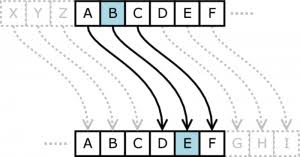
\includegraphics[page=1,width=.5\textwidth]{img/cipher.jpg}
				   \caption{Encoding with shift factor of 3}
		   \label{fig:cipher}
		   \end{figure}
 
 \begin{itemize}
 \item
 "abc " would be encoded to "def"  
 \item
 "haskell is fun" would be encoded to "kdnnhoo lv ixq"

 \end{itemize}
\end{frame}
\begin{frame} [fragile, label = test]

    \frametitle{Caesar Cipher contd..}
More Generally 
\article { the specific shift factor of three used by Caesar can be replaced by any integer between one and twenty-five, thereby giving twenty-five different ways of encoding a string.  So, more generally, with}
With a shift factor of 4, for example:

 \begin{itemize}
 \item
 "abc " would be encoded to "efg"  
  \end{itemize}

We will  use Haskell to implement the Caesar cipher and more.
\end{frame}
 
\pagebreak
\section{Encoding and decoding}
\article{We will use a  number of standard functions on characters that are provided in a 
library called $Data.Char$ which can be loaded into a Haskell script by including the following 
declaration at the start of the script.}
 \begin{frame}[fragile, label=encoding]
  \frametitle{Encoding and Decoding} 
   \begin{onlyenv}
  \begin{lstlisting} [language=Haskell]
 import Data.Char   -- imports standard functions on characters
  \end{lstlisting}
  \end{onlyenv}

    \pause
For simplicity, we will only encode the lower-case characters within a string and leave the other characters unchanged. 
Firstly 
\article { $chr$ and $ord$ are Data.Char functions. $chr$ returns a character given its ordinal number. $ord$ returns a given character's ordinal number. }
  \begin{onlyenv}
  \begin{lstlisting} [language=Haskell]
let2Int :: Char -> Int
let2Int c = ord c - ord 'a' 

int2Let :: Int -> Char
int2Let n = chr (ord 'a' + n)
 \end{lstlisting}
  \end{onlyenv}
\end{frame}

\begin{frame}[fragile, label=encoding2]
 \frametitle{Encoding and Decoding contd. } 
We can see them  called in Figure \ref{int2let}
 \begin{figure} [H]

			\centering
			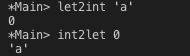
\includegraphics[page=1,width=.5\textwidth]{img/01.png}
				   \caption{ Calling int2let and let2int}
		   \label {int2let}
		   \end{figure}

\end{frame}

 \begin{frame}[fragile, label=encoding2]
  \frametitle{Encoding and Decoding contd. } 
 We define a function \textit{shift} 
 \article {that applies a shift factor to a lower-case letter by converting the letter into the corresponding integer, adding on the shift factor and taking the remainder when divided by 26 (thereby wrapping around the end of the alphabet) and converting the resulting integer back into a lower-case letter. }
 \presentation { as follows: }
 

  \begin{onlyenv}
  \begin{lstlisting} [language=Haskell]
shift :: Int -> Char -> Char
shift n c   | isLower c = int2let ( 
                 (let2int c + n ) `mod` 26)
               | otherwise = c
 \end{lstlisting}
  \end{onlyenv}    
  
  (The library function
   \begin{onlyenv}
  \begin{lstlisting} [language=Haskell]
isLower ::  Char -> Bool
 \end{lstlisting}
  \end{onlyenv}    
returns True if it's a lower-case letter.  )
  \end{frame}

\begin{frame}[fragile, label=encoding3]
  \frametitle{Encoding and Decoding contd. } 
  Using $shift$ within a list comprehension, it is now easy to define a function that encodes a string using a given string factor.
    \begin{onlyenv}
  \begin{lstlisting} [language=Haskell]
encode :: Int -> String -> String 
encode n xs = [shift n x | x <- xs]
 \end{lstlisting}
  \end{onlyenv}    
 
  We call this as shown in Fig \ref{encode}
  
  \begin{figure}
			\centering
			
\includegraphics[page=1,width=.5\textwidth]{img/02.png}
			\caption {Calling encode with positive and negative values}
			\label{encode}
		\end{figure}
\end{frame}


\section{Frequency tables}
\begin{frame}[fragile, label=freq]
\frametitle{Frequency Tables} 
\presentation{
\begin{itemize}
    \item We now look at cracking the Caesar Cipher. 
    \item key - some letters are used more than others in English text.
    \item Analyse a large volume of text, we derive the following table.
\end{itemize}
}
\article{
We now look at cracking the Caesar Cipher. 
The key to this is the observation that some letters are used more frequently than 
others in English text. 
By analysing a large volume of such text one can derive the following table of approximate 
percentage frequencies of the twenty-six letters of the alphabet : 
}
\end{frame}
\begin{frame}[fragile, label=freq]
  \frametitle{Frequency Tables contd.} 
  \presentation  {Table of approximate percentage frequencies of the twenty-six letters of the alphabet : }
    \begin{onlyenv}
  \begin{lstlisting} [language=Haskell]
table :: [Float]
table = [8.1, 1.5, 2.8, 4.1, 12.7, 2.2, 2.0, 
            6.1, 7.0,  0.2, 0.8, 4.0, 2.4, 6.7, 
            7.5, 1.9, 0.1, 6.0, 6.3, 9.0, 2.8, 
            1.0, 2.4, 0.2, 2.0, 0.1]
 \end{lstlisting}
 \end{onlyenv}    

 \article { For example, the letter 'e' occurs most often, with a frequency of 12.7\% while 'q' and 'z' occur least often with a frequency of just 0.1\%. It is also useful to produce frequency tables for individual strings. To this end, we first define a function that calculates the percentage of  one integer with respect to another, returning the result as a floating point number. This function uses fromIntegral which is a library function converts an integer into a floating point number } 
 \presentation { we define a percent function} 
     \begin{onlyenv}
   \begin{lstlisting} [language=Haskell]
percent :: Int -> Int -> Float
percent n m = 
     (fromIntegral n / fromIntegral m ) * 100 
\end{lstlisting}
  \end{onlyenv}    


\end{frame}


\begin{frame}[fragile, label=freq2]
  \frametitle{Frequency Tables cont. } 
  We now look at producing a frequency table for a string. We use $count$ and $lowers$ as follows:
    \begin{onlyenv}
  \begin{lstlisting} [language=Haskell]
count :: Eq a => a-> [a] -> Int
count x xs = length [ x' | x' <- xs, x==x'] 

lowers :: [Char] -> Int
lowers xs = 
     length [x| x <- xs, 
                x >= 'a' && x <= 'z'] 
\end{lstlisting}
 \end{onlyenv}    
\end{frame}


\begin{frame}[fragile, label=freq3]
  \frametitle{Frequency Tables cont. } 
     \begin{onlyenv}
  \begin{lstlisting} [language=Haskell]
freqs :: String -> [Float]
freqs  xs = [percent (count x xs) n | 
                    x <- ['a'..'z']]
      where n = lowers xs
\end{lstlisting}
 \end{onlyenv}    
\pagebreak
  We can see how it's called in Fig \ref{freqs}
  \begin{figure}
			\centering
			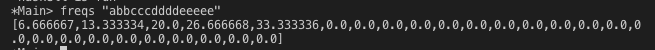
\includegraphics[page=1,width=.9\textwidth]{img/03.png}
			\caption{Calling freqs on a string}
			\label{freqs}
		\end{figure}
\presentation { the letter 'a' occurs with a frequency of approximately 6.6\%, the letter 'b' with a frequency of 13.3\% etc. }
\end{frame}
\article{That is, the letter 'a' occurs with a frequency of approximately 6.6\%, the letter 'b' with a frequency of 13.3\% etc. The use of the $lowers$ function ensures that the percentages are based only on the total number of lower-case letters.}
\section{Cracking the cipher}
\article{A standard method for comparing a list of observed frequencies $os$ with a list of expected frequencies $es$ is the \textit{chi-square statistic}, defined by the following summation in which $n$ denotes the length of the two lists. }
\begin{frame}[fragile, label=freq3]
  \frametitle{Frequency Tables cont. } 
  A standard method for comparing 
  \begin{itemize}
  \item a list of observed frequencies $os$ with 
  \item a list of expected frequencies $es$ 
  \end{itemize}
  is the \textit{chi-square statistic}, defined by the following summation in which $n$ denotes the length of the two lists. 

\[\sum_{i=0}^{n-1} \frac{(os_i - es_i)^2}{es_i}\]
\pause
The smaller the value it produces, the better the match between the two frequency lists.  
\vspace{1cm}
\end{frame}

\begin{frame} [fragile, label = test]
  \frametitle{Frequency Tables cont. } 
Using $zip$ and list comprehension we translate the previous formula into code
 
     \begin{onlyenv}
  \begin{lstlisting} [language=Haskell]
chisqr :: [Float] -> [Float] -> Float
chisqr os es = sum [((o-e)^2)/e | 
                        (o,e) <- zip os es]
\end{lstlisting}
 \end{onlyenv}    
 \end{frame}
 
 \begin{frame} [fragile]
    \frametitle{Frequency Tables cont. } 
 Now, we define a function that rotates the elements of a list $n$ places the left, wrapping around the start of the list, and assuming that the integer arguments $n$ is between 0 and the $length$ of the list 
      \begin{onlyenv}
  \begin{lstlisting} [language=Haskell]
rotate:: Int -> [a] -> [a]
rotate n xs = drop n xs ++ take n xs
\end{lstlisting}
 \end{onlyenv}    
 \pagebreak
\end{frame}
 
\begin{frame} [fragile]
   \frametitle{Frequency Tables cont. } 
Now, suppose that we are given an encoded string, but not the shift factor that was used to encode it, 
and wish to determine this number in order that we can decode the string. 
This can usually be achieved by producing the frequency table of the encoded string, 
calculating the chi-square statistic for each possible rotation of the table with respect to the 
table of expected frequencies, and using the position of the minimum chi-square value as the shift factor. 
\end{frame}
 
\begin{frame} [fragile]
   \frametitle{Frequency Tables cont. } 
For example, if we let table 

\begin{onlyenv}
\begin{lstlisting} [language=Haskell]
table' = freqs "kdvnhoo lv ixq"
\end{lstlisting}
 \end{onlyenv}    

then, 
 
   \begin{onlyenv}
  \begin{lstlisting} [language=Haskell]
[chisqr (rotate' n table') table | n <-  [0..25]]
  \end{lstlisting}
\end{onlyenv}    
   will give us
   \begin{onlyenv}
    \begin{lstlisting} [language=Haskell]
[1409.1558, 639.92175, 612.2969, 202.32024,  1440.2488,  4247.621, 650.89923,  ..]
\end{lstlisting}
 \end{onlyenv}    
 \end{frame}
 \begin{frame} [fragile]
    \frametitle{Cracking the Code}

  \begin{onlyenv}
  \begin{lstlisting} [language=Haskell]
crack :: String -> String 
crack xs = encode (-factor) xs
    where
     factor = head (positions  
     	  ( minimum chitab) chitab ) 
     chitab = [chisqr (rotate' n table') table | 
     	      n <- [0..25]]
     table' = freqs xs
\end{lstlisting}
 \end{onlyenv}    
\end{frame}
%\article {
%[1409.1558,   639.92175,  612.2969,  202.32024,  1440.2488,  4247.621, 650.89923, 1165.0741, 972.48584, 993.0813, 497.77173, 1490.3737, 2296.2412, 1407.7194, 1491.4241, 3033.884, 659.43945, 2836.2344, 986.21796,  809.58765,   1310.7455, 850.54156, 2907.9312, 954.33203, 5313.4775, 626.3024] }
%
 \begin{frame} [fragile]
    \frametitle{Cracking the Code contd.}
For example:
  \begin{onlyenv}
  \begin{lstlisting} [language=Haskell]
crack "kdvnhoo lv ixq"

"haskell is fun"

\end{lstlisting}
 \end{onlyenv}    

 \begin{onlyenv}
  \begin{lstlisting} [language=Haskell]
crack  "vscd mywzboroxcsyxc kbo ecopev" 

"list comprehensions are useful"

\end{lstlisting}
 \end{onlyenv}    



\begin{onlyenv}
 \begin{lstlisting} [language=Haskell]
encode 4 "the cat sat on the mat and the others were in the car"
"xli gex wex sr xli qex erh xli sxlivw aivi mr xli gev"

crack "xli gex wex sr xli qex erh xli sxlivw aivi mr xli gev"
"the cat sat on the mat and the others were in the car"
\end{lstlisting}
\end{onlyenv}    
\end{frame}
\medskip
 
\printbibliography
\end{document}
